\title{Bras mécanique et sudoku}
\author{Laurent Tainturier \& Alphonse TERRIER}
\date{2016-2017}
\documentclass[12pt,a4paper]{report}
\usepackage[utf8]{inputenc}
\usepackage[T1]{fontenc}
\usepackage[french]{babel}
\usepackage{hyperref}
\usepackage{lmodern}
\usepackage{graphicx}
\usepackage{listings}
\usepackage{enumitem}
\usepackage{stmaryrd}
\usepackage{url}
\usepackage{array}
\usepackage{minted}
\usepackage{color}
\usepackage{float}
\usepackage[backend=biber, autolang=other, sorting=none, style=science]{biblatex}
\usepackage[left=4cm,right=3cm,top=2.5cm,bottom=2.5cm]{geometry}
\usepackage{fancyvrb}
\frenchbsetup{StandardLists=true}
\newtheorem{theo}{Définition}[section]
\definecolor{lightgray}{gray}{.6}
\usepackage[dvipsnames]{xcolor}
\definecolor{yellow}{RGB}{225,220,0}
\hypersetup{pdfborder={0 0 0}}

\newenvironment{changemargin}[2]{\begin{list}{}{%
\setlength{\topsep}{0pt}%
\setlength{\leftmargin}{0pt}%
\setlength{\rightmargin}{0pt}%
\setlength{\listparindent}{\parindent}%
\setlength{\itemindent}{\parindent}%
\setlength{\parsep}{0pt plus 1pt}%
\addtolength{\leftmargin}{#1}%
\addtolength{\rightmargin}{#2}%
}\item }{\end{list}}

\usepackage{placeins}

%\addbibresource{bibli.bib}

\begin{document}
\FloatBarrier

\begin{titlepage}
\begin{changemargin}{-1cm}{0cm}
	\centering
	\vspace{5cm}
	{\scshape\huge Institut Supérieur d'Électronique de Paris \par}
	\vspace{1cm}
	{\scshape\LARGE TIPE\par}
	\vspace{1.5cm}
	{\fontsize{45}{45}\selectfont\bfseries Bras mécanique et sudoku\par}
	\vspace{2cm}
	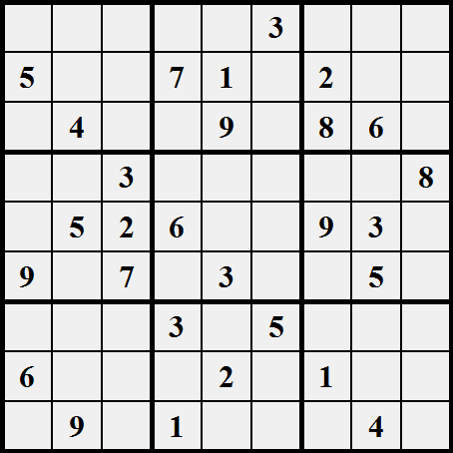
\includegraphics[width=0.7\textwidth]{../pictures/pagedegarde.png}\par\vspace{1.5cm}
	{\LARGE Laurent Tainturier \& Alphonse Terrier\par}
	\vfill
	\large supervisé par\par
	\large \bfseries M. Patrick COUVEZ

	\vfill

	{\large 2016-2017}
\end{changemargin}
\end{titlepage}

\tableofcontents
\addcontentsline{toc}{chapter}{Introduction}
	\chapter*{Introduction}
	

	\chapter{Présentation et faits sur le sudoku}
	
	Le sudoku est un jeu sous forme de grille inspiré du carré latin et défini en 1979 par Howard Garns.
	
	Cette grille est carrée et est divisée en $n^2$ régions de $n^2$ cases. Elle possède ainsi $n^2$ colonnes, $n^2$ lignes et $n^4$ cases. Dans la version la plus commune : $n=3$.

Une grille de sudoku est préremplie, le but du jeu étant de la compléter selon la règle suivante :
\begin{itemize}[label=--]
\item Chaque ligne, chaque colonne et chaque région doit contenir au moins une fois tous les de $1$ à $n^2$.
\end{itemize} 

Une grille est considérée comme sudoku seulement si sa solution est unique.

Le minimum de cases remplies au préalable pour espérer que la dite solution soit bien unique est de 17, cela a été prouvé par une équipe islandais en 2012.

	\chapter{Électronique}
\section{Moteurs pas-à-pas}
Nous avons utilisés dans ce projet deux moteurs pas-à-pas qui présentaient, par rapport à d'autres types de moteurs, les avantages suivants : 
\begin{itemize}[label=--]
\item une précision bien supérieure à celle de moteurs à courant continu;
\item un couple bien plus important que celui de servomoteurs;
\item mis sous tension, un déplacement fortuit du moteur n'est pas possible.
\end{itemize}
Les moteurs pas-à-pas sont notamment utilisés dans les systèmes nécessitant une grande précision comme les imprimantes 3D dans lesquelles ils sont très largement employés.

\section{Schéma électrique}
Le schéma ci-joint représente les principales connections au sein de notre montage, même s'il ne présente ni l'écran LCD, ni le détail de l'alimentation (notamment du convertisseur de tension).

Les moteurs pas-à-pas sont constitués de deux bobines qui sont reliées à deux drivers l293D . Ceux-ci sont pilotés par quatre sorties GPIO qui envoient des impulsions au driver qui alimente les bobines en 12V à tour de rôle, ce qui permet à la fois de contrôler le sens et la vitesse de de rotation des moteurs, en choisissant à quelle fréquence envoyer les impulsions.
\begin{figure}[!h]
 \center
 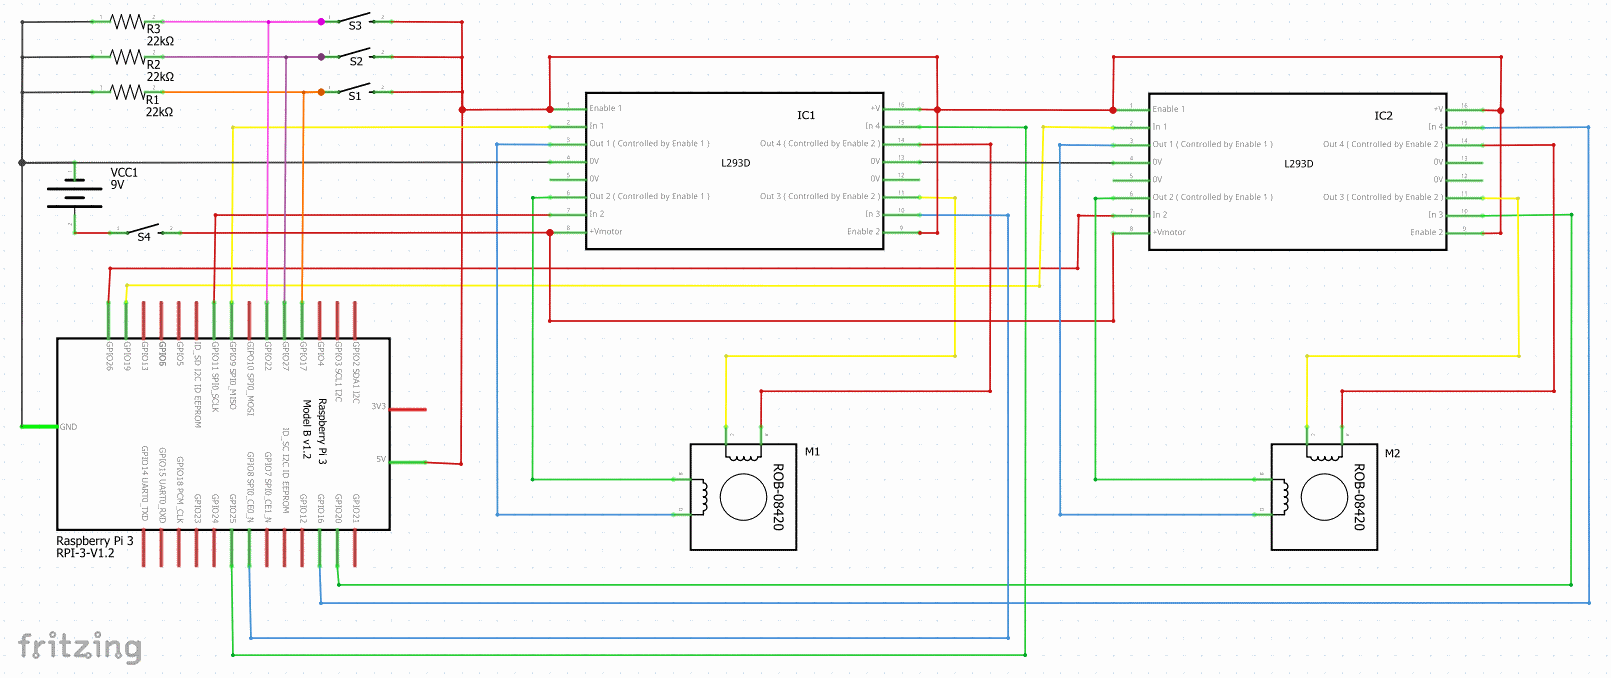
\includegraphics[scale=0.34]{../pictures/Sudoku_schema_electrique.png}
 \caption{Schéma électrique réalisé avec \emph{Fritzing}}
\end{figure}

\section{Premiers montages}
Nous avons réalisés nos premiers montages avec une breadboard facilitant les tests. Une simulation du schéma a également été réalisée sous \emph{Fritzing}
\begin{figure}[!h]
 \center
 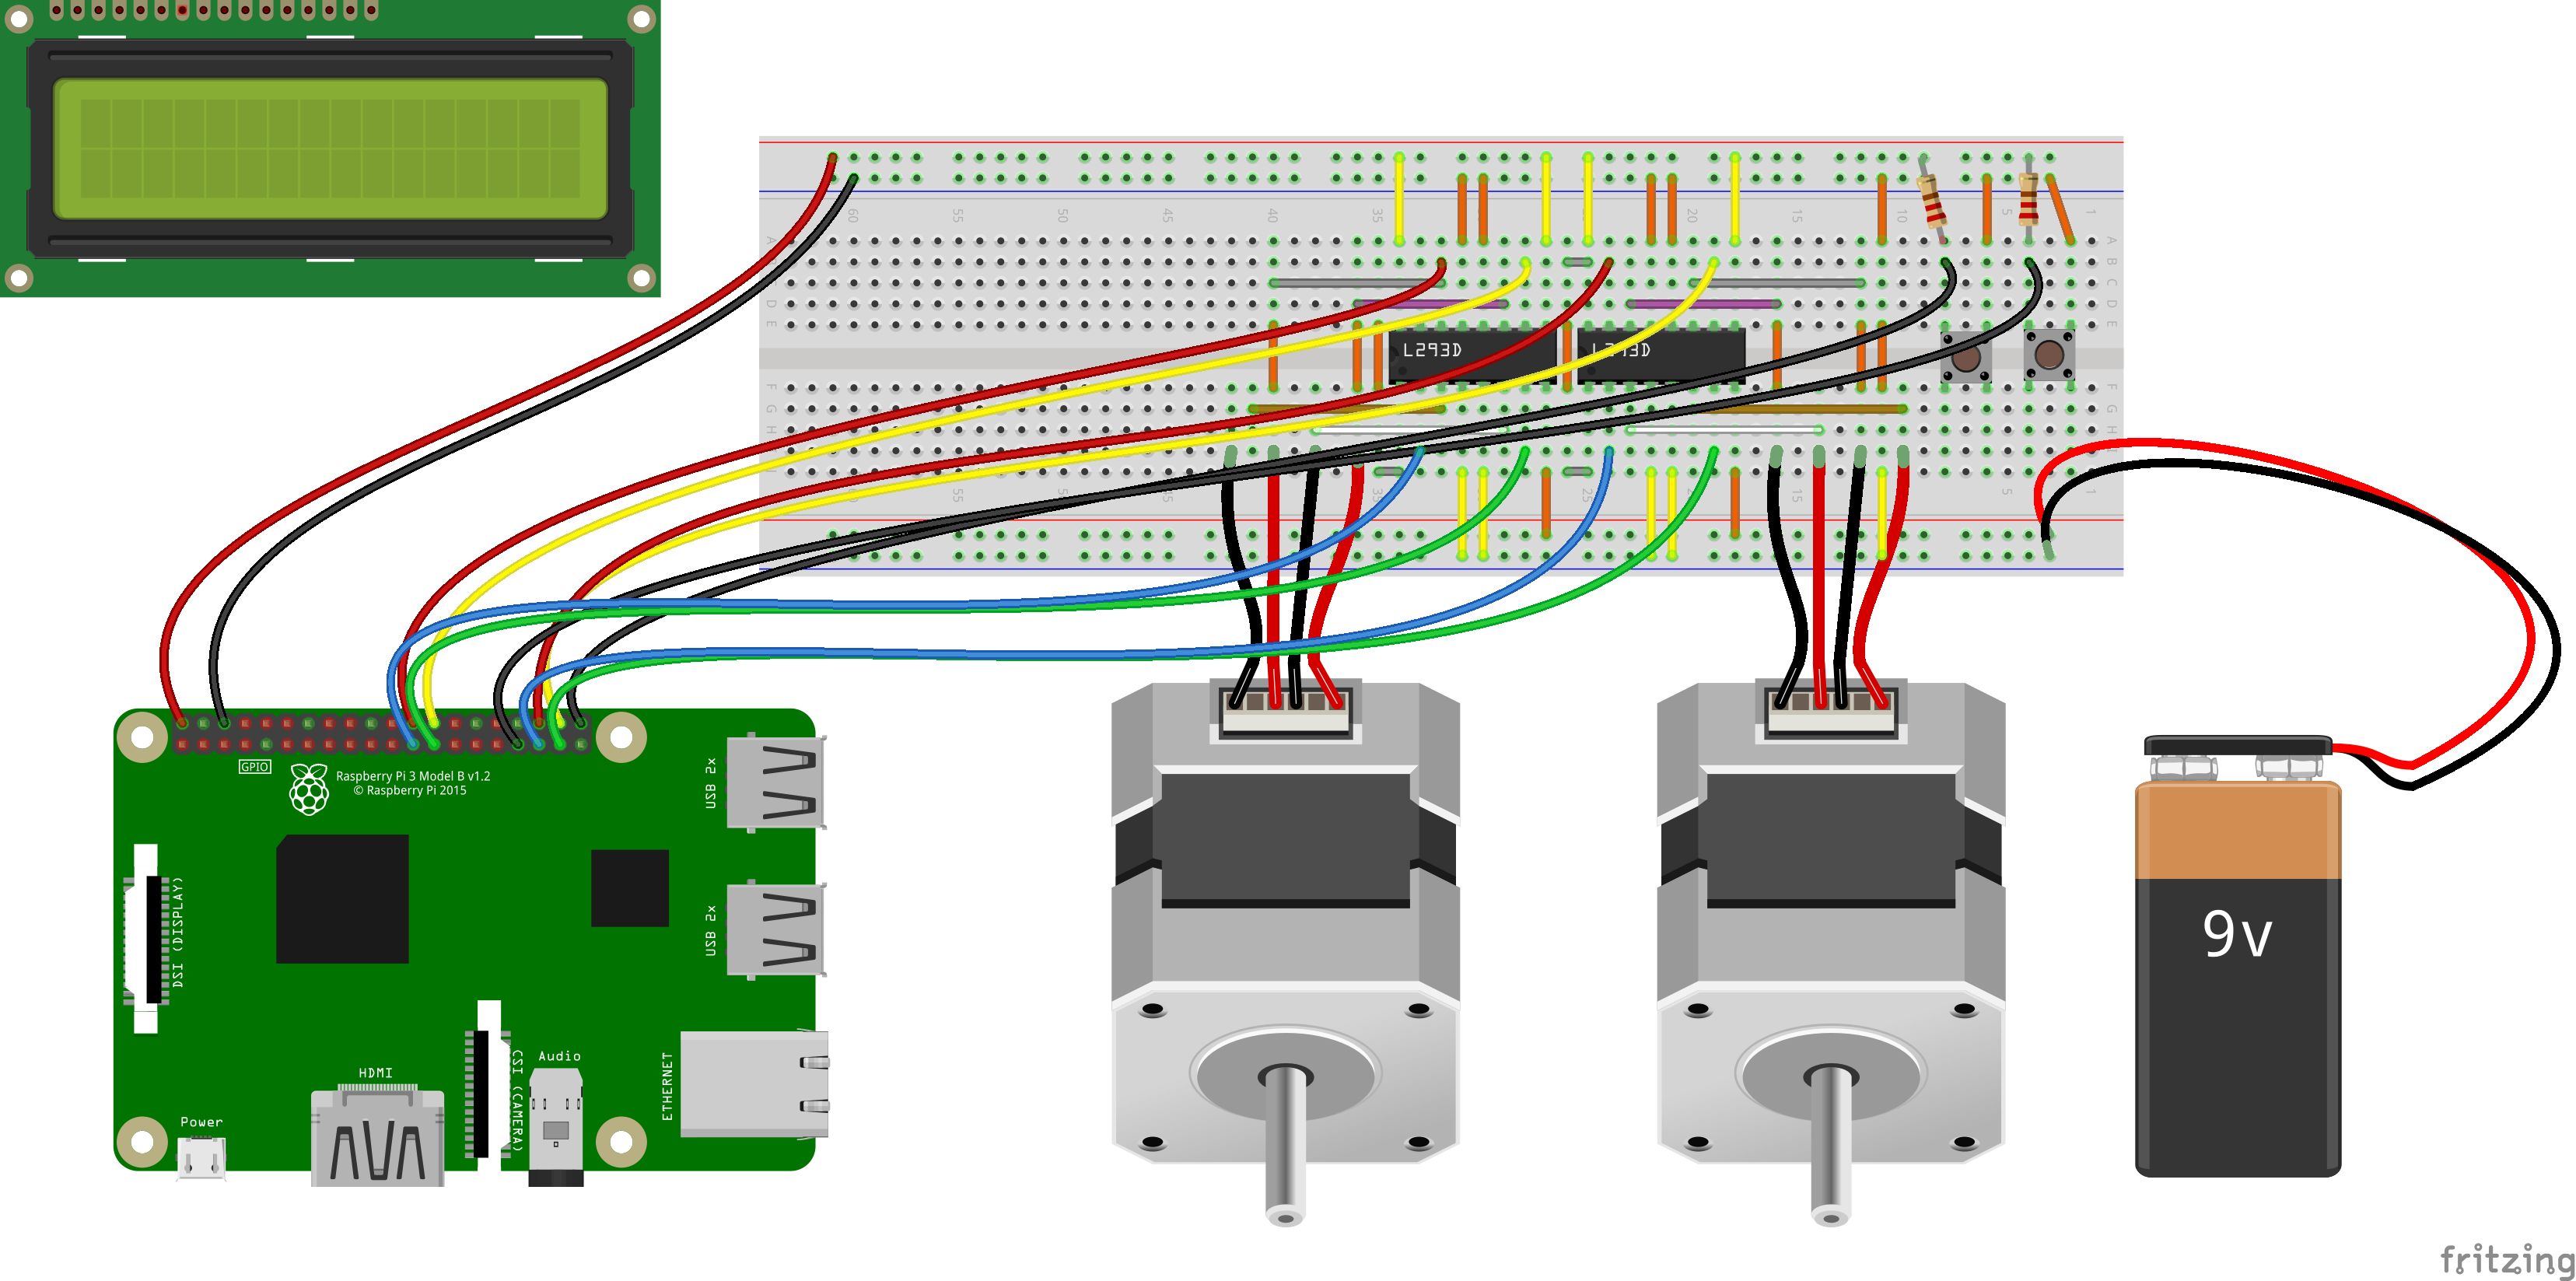
\includegraphics[scale=0.45]{../pictures/Sudoku_schema}
 \caption{Premier montage}
\end{figure}

\section{Circuit imprimé}
Pour rendre notre bras mécanique plus compact et ainsi rentrer dans le cadre de l'optimalité, nous avons souhaité remplacé la breadboard par une solution bien plus compacte, à savoir un circuit imprimé. Celui-ci sera enficher directement sur les ports GPIO de la Raspberry. Nous avons de nouveau utilisé pour le réaliser le logiciel \emph{Fritzing}, permettant la réalisation du circuit sur deux couches (symbolisées par les couleurs orange et jaune), permettant un cablage plus facile, car permettant les croisements. Nous avons utilisé \emph{Fritzing} car il été assez facile de faire faire fabriquer le circuit imprimé pour une dizaine d'euros. Nous avions hésité à réaliser entièrement ce circuit par nous même, mais du fait de la présence de deux couches, cela se serait révéler très difficile.

\begin{figure}[!h]
 \center
 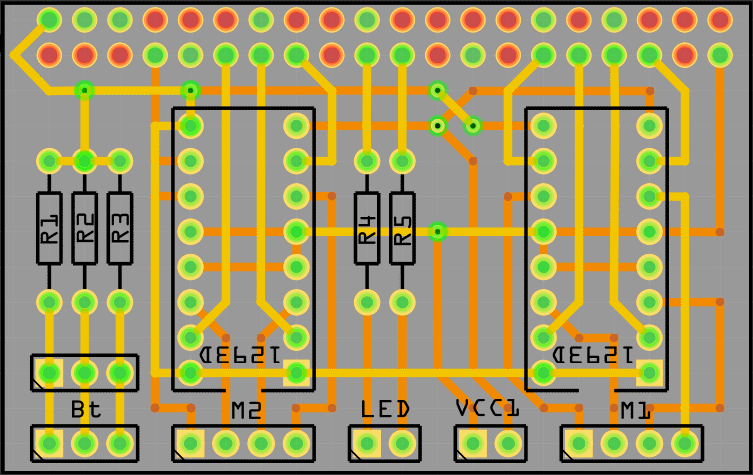
\includegraphics[scale=0.5]{../pictures/Sudoku_circuit_imprime.png}
 \caption{Circuit imprimé réalisé avec \emph{Fritzing}}
\end{figure}

\section{Écran LCD}
Pour rendre le bras mécanique autonome, nous avons intégré un écran LCD permettant à l'utilisateur de se repérer dans l'évolution des différents scripts sans disposer nécessairement d'un ordinateur ou d'un écran à proximité.
\begin{figure}[!h]
 \center
 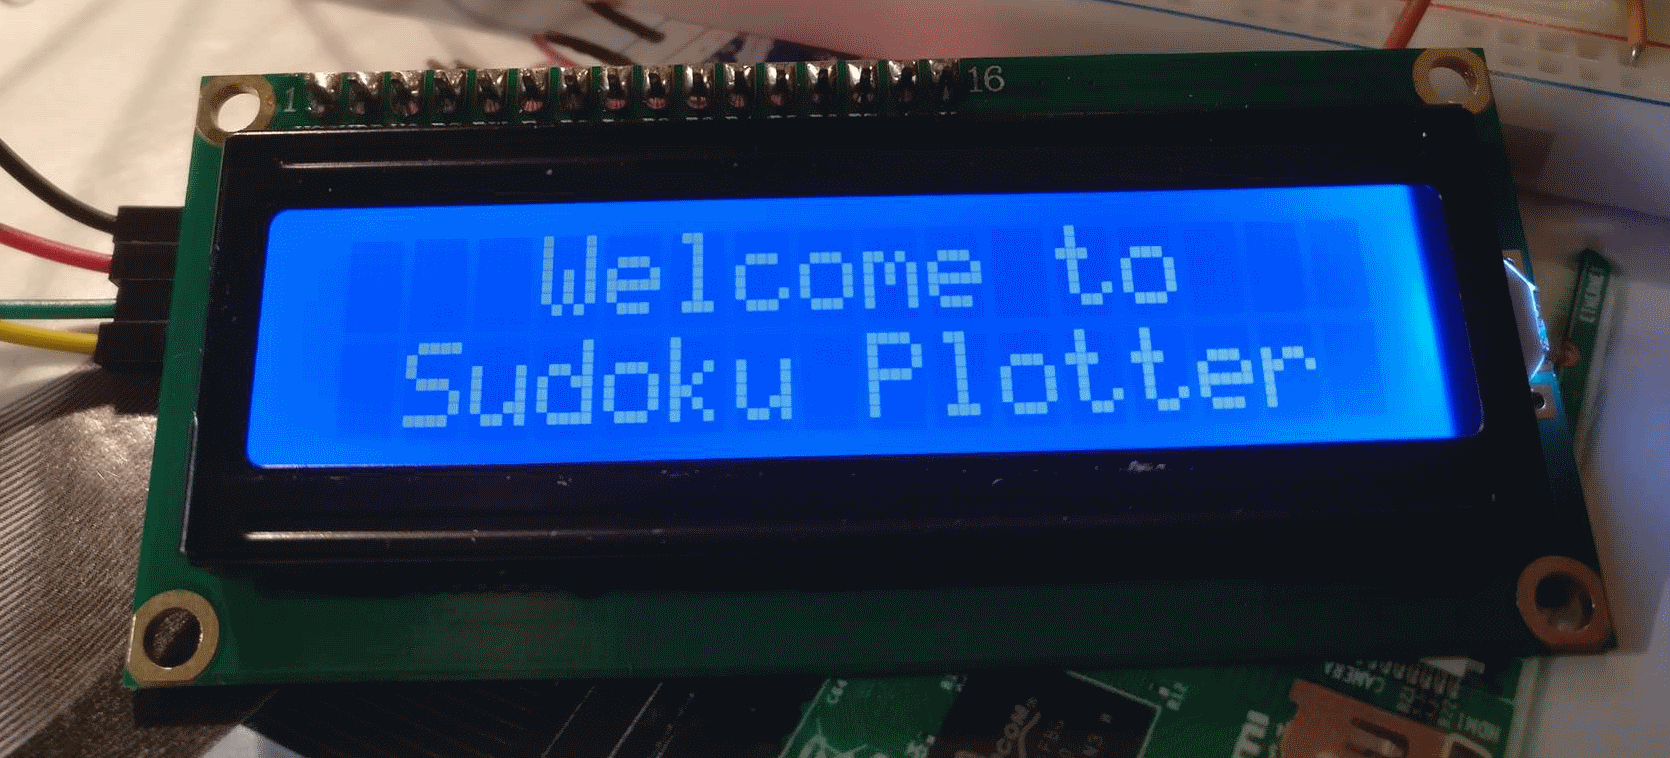
\includegraphics[scale=0.3]{../pictures/ecran_lcd}
 \caption{\'{E}cran LCD affichant le message de bienvenue}
\end{figure}

	\chapter{Mécanique}
	
	La premier défi qui s'est imposé à nous a été le choix d'une structure adéquate : solide et pratique. Notre choix s'est alors porté sur les Makerbeam. MakerBeam est un système de construction Open-Source basé sur des profilés ALU en T.
	
	L'écriture se fera en coordonnées polaires et non pas en coordonnées cartésiennes pour les raisons suivantes :
	\begin{itemize}[label=--]
	\item un système en coordonnées cartésiennes aurait été trop encombrant et un moins "portable" (dans un contexte notamment d'optimalité, comme exigé par le programme)
	\item c'est un défi technique de fabriquer un bras de ce type en coordonnées polaires
	\end{itemize}
	
Ainsi, un moteur pas-à-pas assurera la rotation $\theta$ du bras. Ce moteur s'auto-entrainera autour d'une roue dentée de 128 dents comme celle-ci et un roulement permettra la rotation de l'entièreté du bras :

\begin{figure}[!h]
 \center
 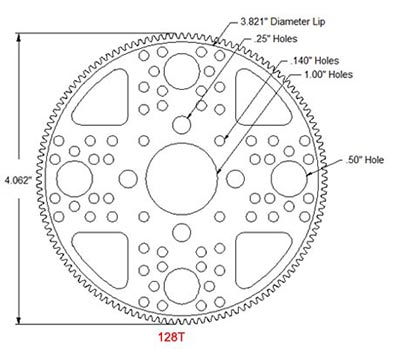
\includegraphics[scale=0.5]{../pictures/rouedentee2.jpg}
 \caption{Schéma de la roue dentée}
\end{figure}


De même la translation $r$ a été assurée par un deuxième moteur pas-à-pas et un système courroie/poulie. Cette translation s'est faite le long de deux axes de $272$ mm et de $8$ mm de diamètre.
	\section{Difficultés rencontrées et solutions mises en place}
	Nous avons notamment rencontré des difficultés concernant le roulement utilisé. En effet, nous avions au préalable utilisé un roulement à billes comme celui-ci :
	
	\begin{figure}[!h]
 \center
 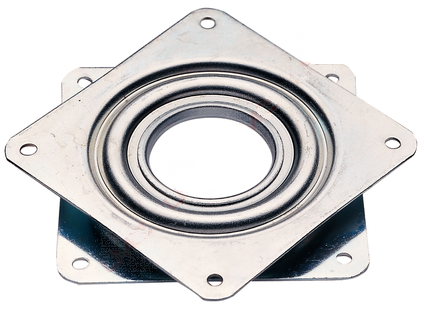
\includegraphics[scale=0.5]{../pictures/roulementmerdique}
 \caption{Roulement défectueux}
\end{figure}

Malheureusement, ce roulement tournait très mal et saccadait. De plus, du jeu était présent. Après quelques heures de recherche, nous avons donc choisi le roulement à billes suivant, qui tourne très bien mais qui tout de même possède lui aussi un peu de jeu :

	\begin{figure}[!h]
 \center
 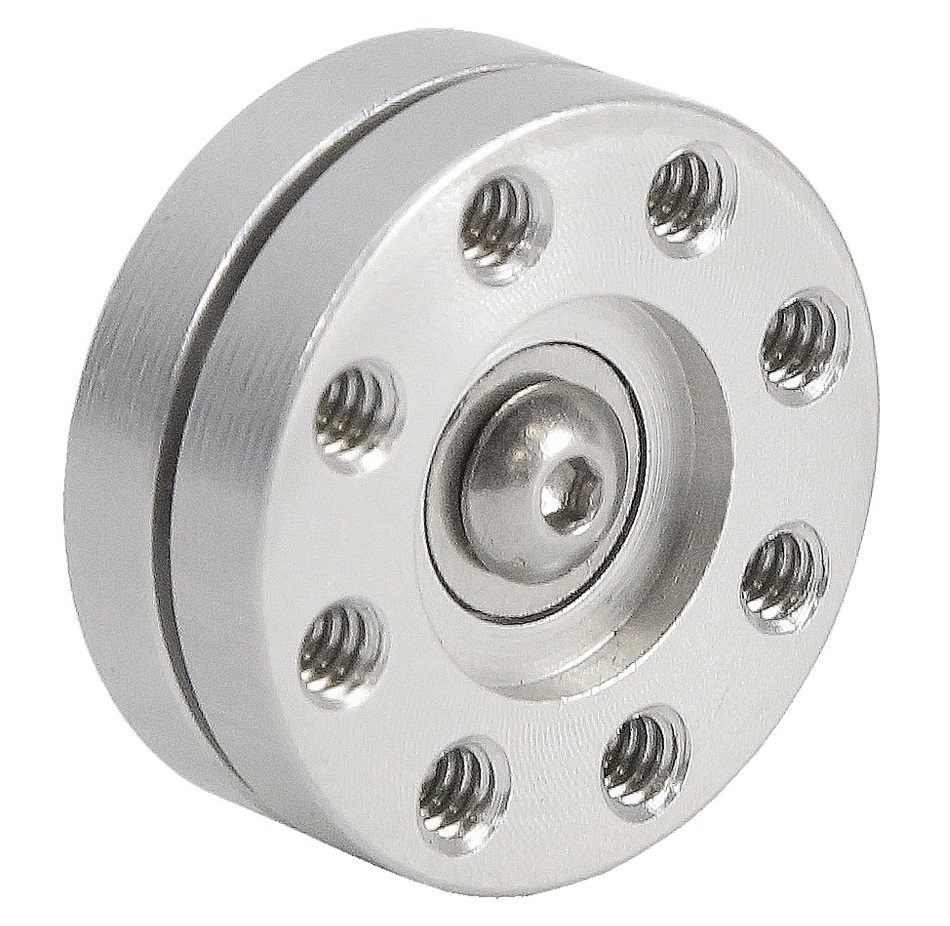
\includegraphics[scale=0.15]{../pictures/swivelhub}
 \caption{Roulement finalement choisi}
\end{figure}

	
	
	\section{Conception du chariot en 3D}
	
	Nous avons pris la décision de concevoir certaines pièces de notre projet en 3D, celle-ci nécessitant de la précision. Le logiciel professionnel de modélisation SolidWorks a été utilisé pour développer ces pièces.
	
	Les mises en plan des pièces composant le chariot sont disponibles en annexe \ref{chariot} à partir de la page \pageref{chariot}.
	
	La partie principale du chariot devait pouvoir accueillir un servomoteur, permettant l'abaissement et le soulèvement du stylo :
	
	%\begin{figure}[!h]
 %\center
 %\includegraphics[scale=0.15]{../pictures/chariot}
 %\caption{Impression 3D de la pièce principale du chariot}
	%\end{figure}
	
	Ce stylo sera fixé sur la pièce présentée en page\pageref{supportstylo} dont l'impression 3D est montrée ci-dessous :
	
	%\begin{figure}[!h]
 %\center
 %\includegraphics[scale=0.15]{../pictures/supportstylo}
 %\caption{Impression 3D de la pièce supportant le stylo}
	%\end{figure}
	
L'ensemble chariot/support du stylo imprimé en 3D est alors montrée ci-dessous :

	%\begin{figure}[!h]
 %\center
 %\includegraphics[scale=0.15]{../pictures/supportchariot}
 %\caption{Impression 3D du chariot et du support du stylo}
	%\end{figure}

Le chariot permet, de façon modulaire, d'accueillir un support caméra se divisant en deux pièces présentées en page \pageref{chariotcamera} et en page \pageref{supportcamera}.
	
	\chapter{Informatique}
\section{Présentation globale}
	Tous les algorithmes développé dans le cadre de ce projet sont disponibles en annexe. Ils ont été, pour la plupart, développé en Python 3, les autres se basant sur Python 2 car certaines bibliothèques dont nous avions besoin, notamment pour la reconnaissance, n'était disponible que sous Python 2. 
	
	Nous avons développé une programmation modulaire, permettant de travailler simultanément sur le projet, sans pour autant poser de problème de logistique. Ainsi nous avons dissocié tous les scripts ; que ce soit la reconnaissance, la résolution, l'affichage, la gestion de la caméra ou des servo-moteurs, etc. Pour cela, nous avons développé une relation qualifiable de maître-esclave entre nos scripts. Chacun des scripts dépend d'un fichier principal, appelé \emph{main}, qui récupère les informations des scripts et donne les ordres adéquats à ceux-ci, selon la situation. Ainsi, les scripts ne sont pas reliés les uns aux autres mais seulement à ce script principal, ce qui permet d'ajouter ou d'enlever très facilement tel ou tel script, sans pour autant altérer le fonctionnement de l'ensemble, ce qui permet de tester chacun des scripts très facilement.
	
\section{Reconnaissance du sudoku}
	Le script de reconnaissance du sudoku a été réalisé sous Python 2 avec le module de traitements d'image OpenCV. Il a été réalisé pour :
	\begin{itemize}[label=--]
	\item Reconnaître les chiffres dans une grille du sudoku
	\item Déterminer la position spatiale de la grille
	\end{itemize}
	\newpage
	On photographie la grille avec une caméra Raspberry Pi (V2) comme celle-ci :
	\begin{figure}[!h]
 \center
 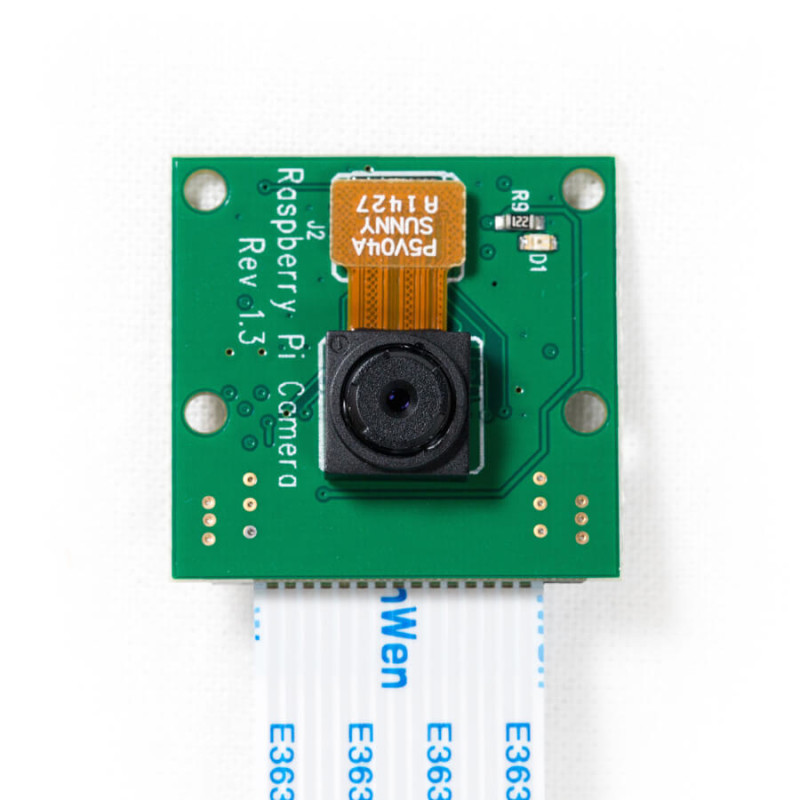
\includegraphics[scale=0.2]{../pictures/camera.jpg}
 \caption{Caméra Raspberry Pi V2}
\end{figure}

Voici la grille de sudoku qui nous servira d'exemple pour montrer toutes les actions du script :
\begin{figure}[!h]
 \center
 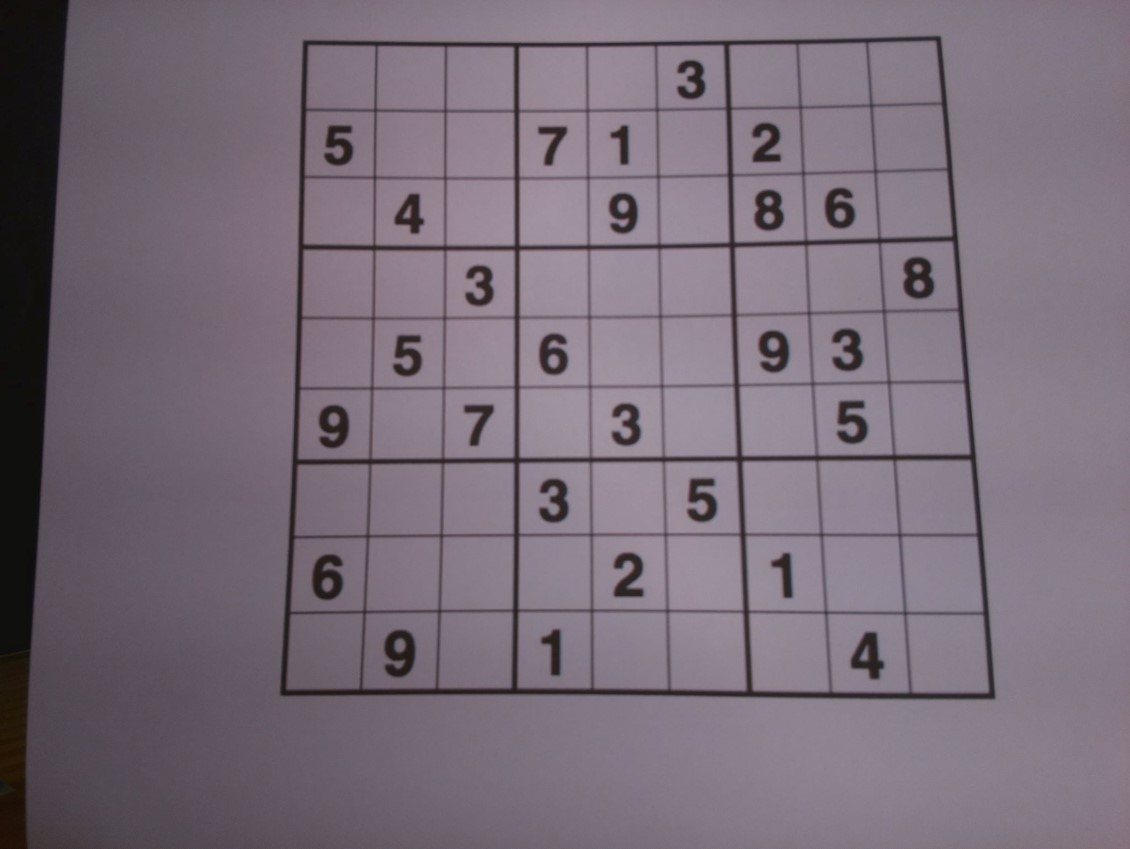
\includegraphics[scale=0.2]{../pictures/example.jpg}
 \caption{Exemple de grille de sudoku}
\end{figure}

On applique sur cette photographie un filtre de type seuil (en anglais "threshold") qui va ensuite nous permettre de détecter les contours de la grille :

\begin{figure}[!h]
 \center
 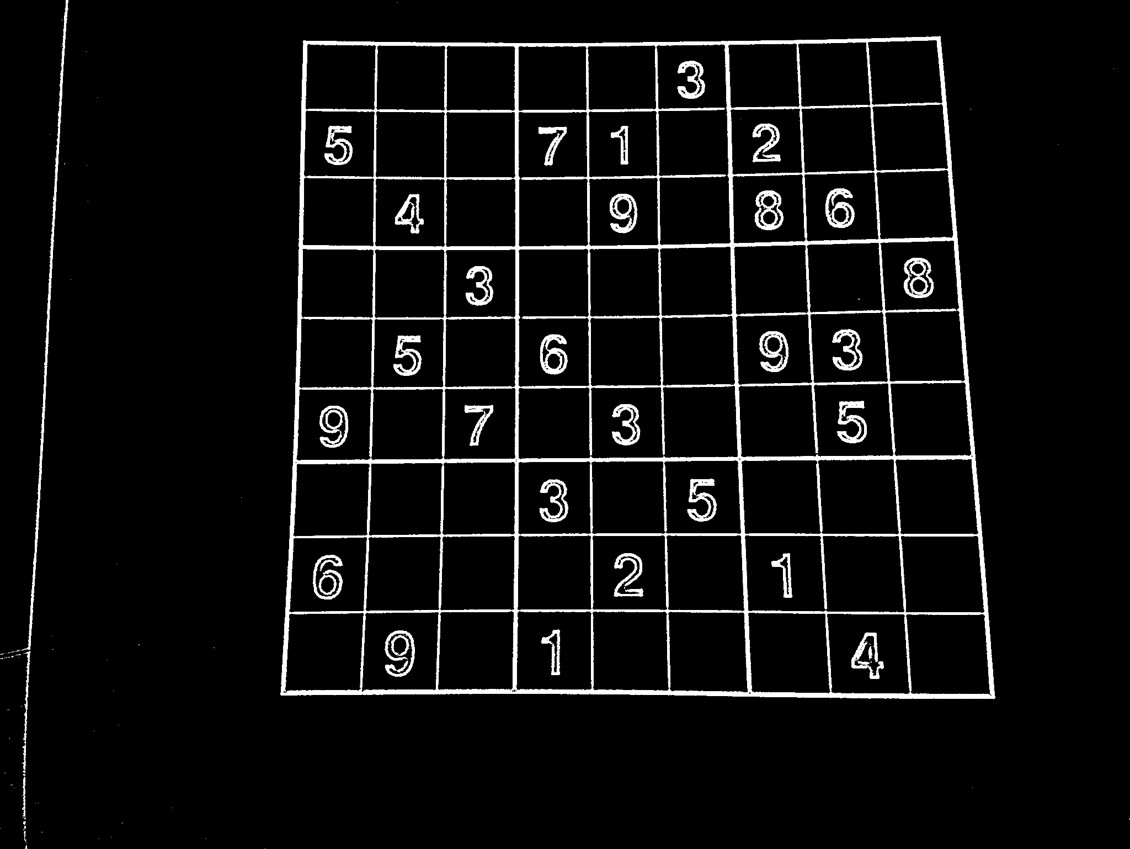
\includegraphics[scale=0.2]{../pictures/threshold.jpg}
 \caption{Exemple de grille "seuillée"}
 \end{figure}
 
Par cette transformation, on peut ensuite déterminer des équations de droites des contours extérieurs de la grille. Les coordonnées des intersections des droites seront celle des coins de la grille. \smallbreak On découpe alors la grille de la photographie initiale en supprimant les éventuels effets de perspective. 
 
\begin{figure}[!h]
 \center
 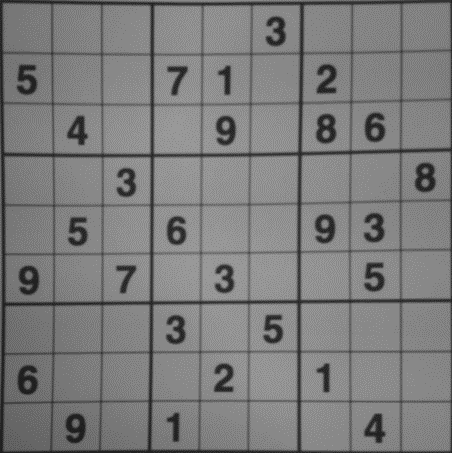
\includegraphics[scale=0.45]{../pictures/unperspectived.png}
 \caption{Exemple de grille découpée sans perspective}
\end{figure}

On découpe chaque petite case de la grille comme ci-dessous :

\begin{figure}[!h]
 \center
 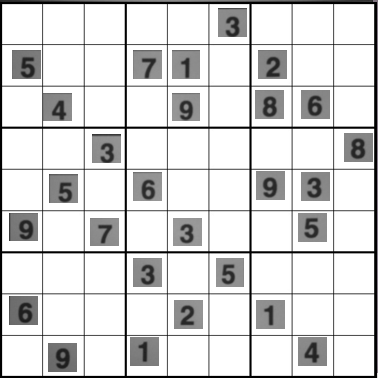
\includegraphics[scale=0.5]{../pictures/cutted.png}
 \caption{Exemple de grille où chaque chiffre a été découpé}
\end{figure}

On utilise ensuite un module de reconnaissance de digits pour détecter les chiffres et on obtient la grille suivante, prête à être résolue :

\begin{figure}[!h]
 \center
 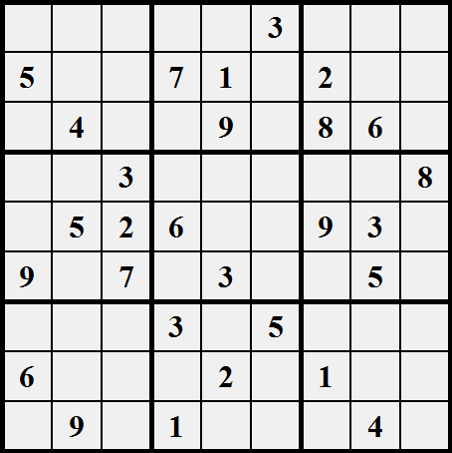
\includegraphics[scale=0.45]{../pictures/finished.png}
 \caption{Exemple de grille prête à être résolue}
\end{figure}
\newpage

\section{Résolution du sudoku}
\label{Resolution}
Pour résoudre une grille de sudoku, un joueur utilise différentes méthodes de résolution, qui sont purement algorithmiques. Il utilise en grande majorité deux principales méthodes qui peuvent permettre de résoudre une grande partie des grilles disponibles sur le marché. On appelle ces deux méthodes \emph{inclusion} et \emph{exclusion}. Cependant les grilles de niveau supérieur font appel à des méthodes plus subtiles et souvent plus difficiles à appliquer en pratique qui se basent généralement sur des \emph{paires} ou des \emph{triplets}. Enfin, il existe une méthode, très difficilement utilisable par un joueur, appelée \emph{backtracking} (en français : \emph{retour sur trace}), qui permet de résoudre toute grille de sudoku, même si celle-ci possède plusieurs solutions.
\paragraph{Inclusion}
\paragraph{Exclusion}
\paragraph{Paires} Cette méthode possède différentes variantes :
\begin{itemize}[label=--]
\item 
\item
\end{itemize} 
La méthode des triplets est une généralisation de cette méthode à trois cases et non seulement deux.
\paragraph{Backtracking} Cette méthode consiste tout d'abord à lister pour chacune des cases vierges les chiffres qui pourraient correspondre. On part d'une case vierge quelconque qu'on remplit par un des chiffres qu'on pourrait théoriquement placer et on liste de nouveau les possibilités des autres cases en fonction du chiffre précédemment ajouté puis on passe à une autre case vierge. S'il n'y a plus aucune possibilités qui pourraient correspondre, on revient sur nos pas et on change le chiffre qu'on venait d'insérer en une autre possibilité. S'il n'y a plus de possibilités, on revient de nouveau sur nos pas autant de fois que nécessaire jusqu'à avoir compéter la totalité de la grille.

\section{Interface graphique}
Pour rendre la résolution plus simple d'utilisation, nous avons décidé d'ajouter une interface graphique. Le cahier des charges qu'elle devait vérifier était assez stricte. Elle devait pouvoir afficher, avant toute chose, une grille de sudoku qui devait dès lors être facilement modifiable. Pour cela, nous avons donc créé différents menus ; l'un permettant donc l'édition de la grille, un autre permettant de choisir la méthode de résolution, ainsi qu'un menu de résolution. 

\paragraph{Édition} Lors de l'édition de la grille, un carré rouge apparait, déplaçable avec les flèches directionnelles, il suffit alors pour modifier la case de rentrer un chiffre de 0 à 9, 0 correspondant à une case vierge. Il est également possible de sauvegarder une grille ou encore de récupérer une grille déjà enregistrée.

\begin{figure}[!h]
 \center
 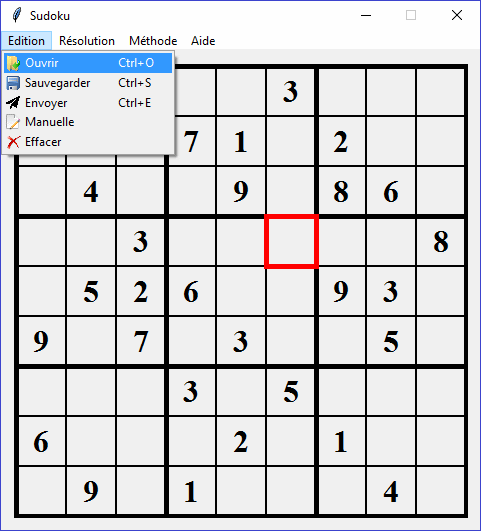
\includegraphics[scale=0.5]{../pictures/Sudoku_edition}
 \caption{Interface graphique affichant le menu Edition}
\end{figure}

\paragraph{Résolution}Ce menu permet de lancer la résolution, et permet également de choisir entre une résolution rapide ou une résolution pas-à-pas permettant à l'utilisateur d'observer le fonctionnement de ces algorithmes.

\begin{figure}[!h]
 \center
 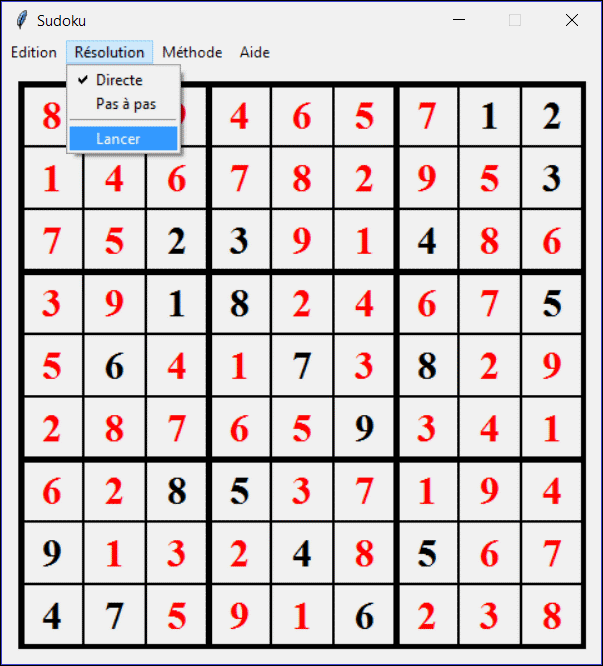
\includegraphics[scale=0.5]{../pictures/Sudoku_resolution}
 \caption{Interface graphique affichant le menu Édition}
\end{figure}

\paragraph{Méthode}Le choix de la méthode se fait avec le menu \emph{Méthode}, qui permet de choisir la méthode de résolution parmi l'\emph{inclusion}, l'\emph{exclusion} et le \emph{backtracking} \footnote{cf section~\ref{Resolution} à la page \pageref{Resolution}} ou de choisir une méthode dite \emph{globale}, s'appuyant sur tous les algorithmes, permettant ainsi d'être la plus rapide possible.

\section{Contrôle des moteurs et écriture}
\subsection*{Moteurs pas-à-pas}

\subsection*{Coordonnées polaires}
Par soucis de compacité, nous avons décidé de développer une structure se basant sur les coordonnées cylindriques, permettant des dimensions maximum de 40 par 10 cm au lieu de 40 par 40 en coordonnées cartésiens. En effet, en coordonnées cartésien, pour rendre le système stable, il aurait fallu placer une tige de chaque côté de la feuille, sur lesquelles se déplacerait une plateforme pouvant déplacer le stylo selon la largeur de la feuille. De plus, l'utilisation des coordonnées polaires ne sont que très peu utilisés pour ce type de système, ce qui se révélait donc plus intéressant à développer.
\begin{figure}[!h]
 \center
 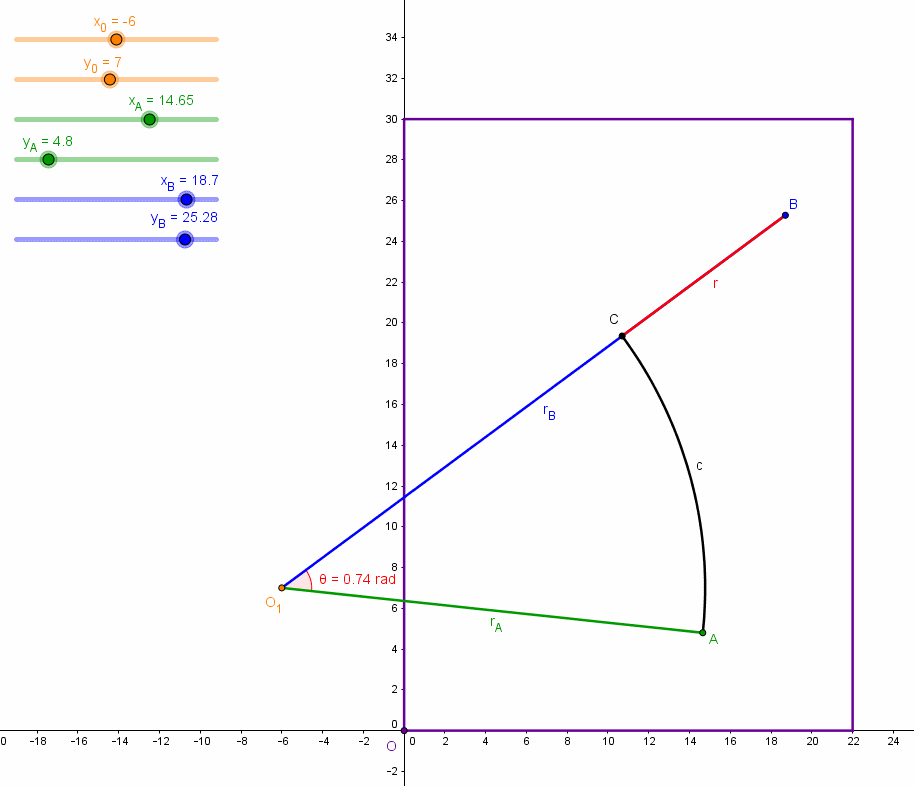
\includegraphics[scale=0.5]{../pictures/Changement_repere}
 \caption{Changement de repères réalisé avec \emph{Geogebra}}
\end{figure}

\subsection*{Écriture des digits}
Nous souhaitions dès le début pouvoir écrire des grilles de différentes tailles, et non des grilles de tailles fixes. C'est pourquoi nous avons basé le script d'écriture sur du point par point, permettant de choisir la précision théorique des chiffres tracés. Cependant les moteurs pas-à-pas ne pouvant se déplacer que d'un pas fixé de 1.8\degre, une trop grande précision ne pourrait entraînerait que des déplacements nuls des moteurs, c'est pourquoi cette manière de programmation permet un compromis entre précision théorique et précision pratique.
\begin{figure}[!h]
 \center
 
\includegraphics[scale=0.35]{../pictures/numbers}
 \caption{Chiffres d'une précision théorique assez faible}
\end{figure}

En augmentant la précision théorique, on obtient des chiffres quasiment continus permettant d'obtenir la figure suivante.

\begin{figure}[!h]
 \center
 \includegraphics[scale=0.5]{../pictures/Sudoku_points}
 \caption{Grille de sudoku en point par point tracée avec \emph{MatplotLib}}
\end{figure}

Il faut prévoir dans le script la possibilité d'envoyé une impulsion au servomoteur afin qu'il lève le stylo lorsqu'un chiffre a été tracée afin d'éviter que les chiffres ne soient reliés entre eux, comme le suggère la figure suivante.

\begin{figure}[!h]
 \center
 \includegraphics[scale=0.5]{../pictures/Sudoku_relies}
 \caption{Grille de sudoku tracée avec \emph{MatplotLib}}
\end{figure}

\chapter*{Conclusion}
Tous les scipts et ce dossier sont disponibles sur GitHub\footnote{\url{www.github.com/alphter/Sudoku-Plotter/}}

\chapter*{Remerciements}

Nous remercions M. Couvez pour ses précieux conseils et Tristan Vajente pour les impressions de pièces en 3D.

\printbibliography
\nocite{*}
\appendix

\begin{changemargin}{-2cm}{-4cm}

\addcontentsline{toc}{chapter}{Scripts Python}
\label{Scripts}
\chapter*{Script principal}
\label{main}
%\inputminted[fontsize=\scriptsize, linenos=true]{Python}{../script/main.py}

\chapter*{Script de résolution des sudokus}
\label{resolution}
%\inputminted[fontsize=\scriptsize, linenos=true]{Python}{../script/resolution.py}

\chapter*{Script de gestion de la caméra}
\label{camera}
%\inputminted[fontsize=\scriptsize, linenos=true]{Python}{../script/camera.py}

\chapter*{Script d'affichage du sudoku}
\label{display}
%\inputminted[fontsize=\scriptsize, linenos=true]{Python}{../script/display.py}

\chapter*{Script de gestion des moteurs pas-à-pas}
\label{step_motor}
%\inputminted[fontsize=\scriptsize, linenos=true]{Python}{../script/step_motor.py}

\chapter*{Script permettant l'écriture d'un sudoku}
\label{write}
%\inputminted[fontsize=\scriptsize, linenos=true]{Python}{../script/write.py}
\addcontentsline{toc}{chapter}{Mises en plan des pièces conçues en 3D}

\chapter*{Mise en plan du chariot}
\begin{figure}[!h]
 \center
 \includegraphics[scale=1]{../3Dmodels/chariot.png}
\end{figure}

\chapter*{Mise en plan du support du stylo}
\begin{figure}[!h]
 \center
 \includegraphics[scale=1]{../3Dmodels/supportstylo.png}
\end{figure}

\chapter*{Mise en plan du lien chariot/caméra}
\begin{figure}[!h]
 \center
 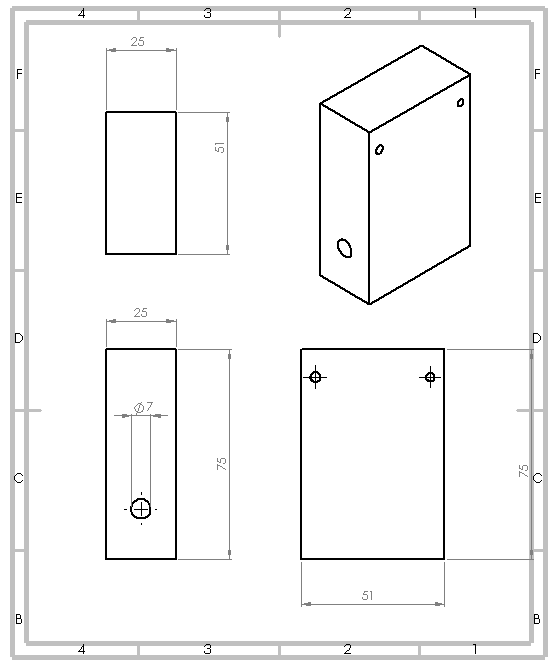
\includegraphics[scale=0.95]{../3Dmodels/camerachariot.png}
\end{figure}

\chapter*{Mise en plan du support de la caméra}
\begin{figure}[!h]
 \center
 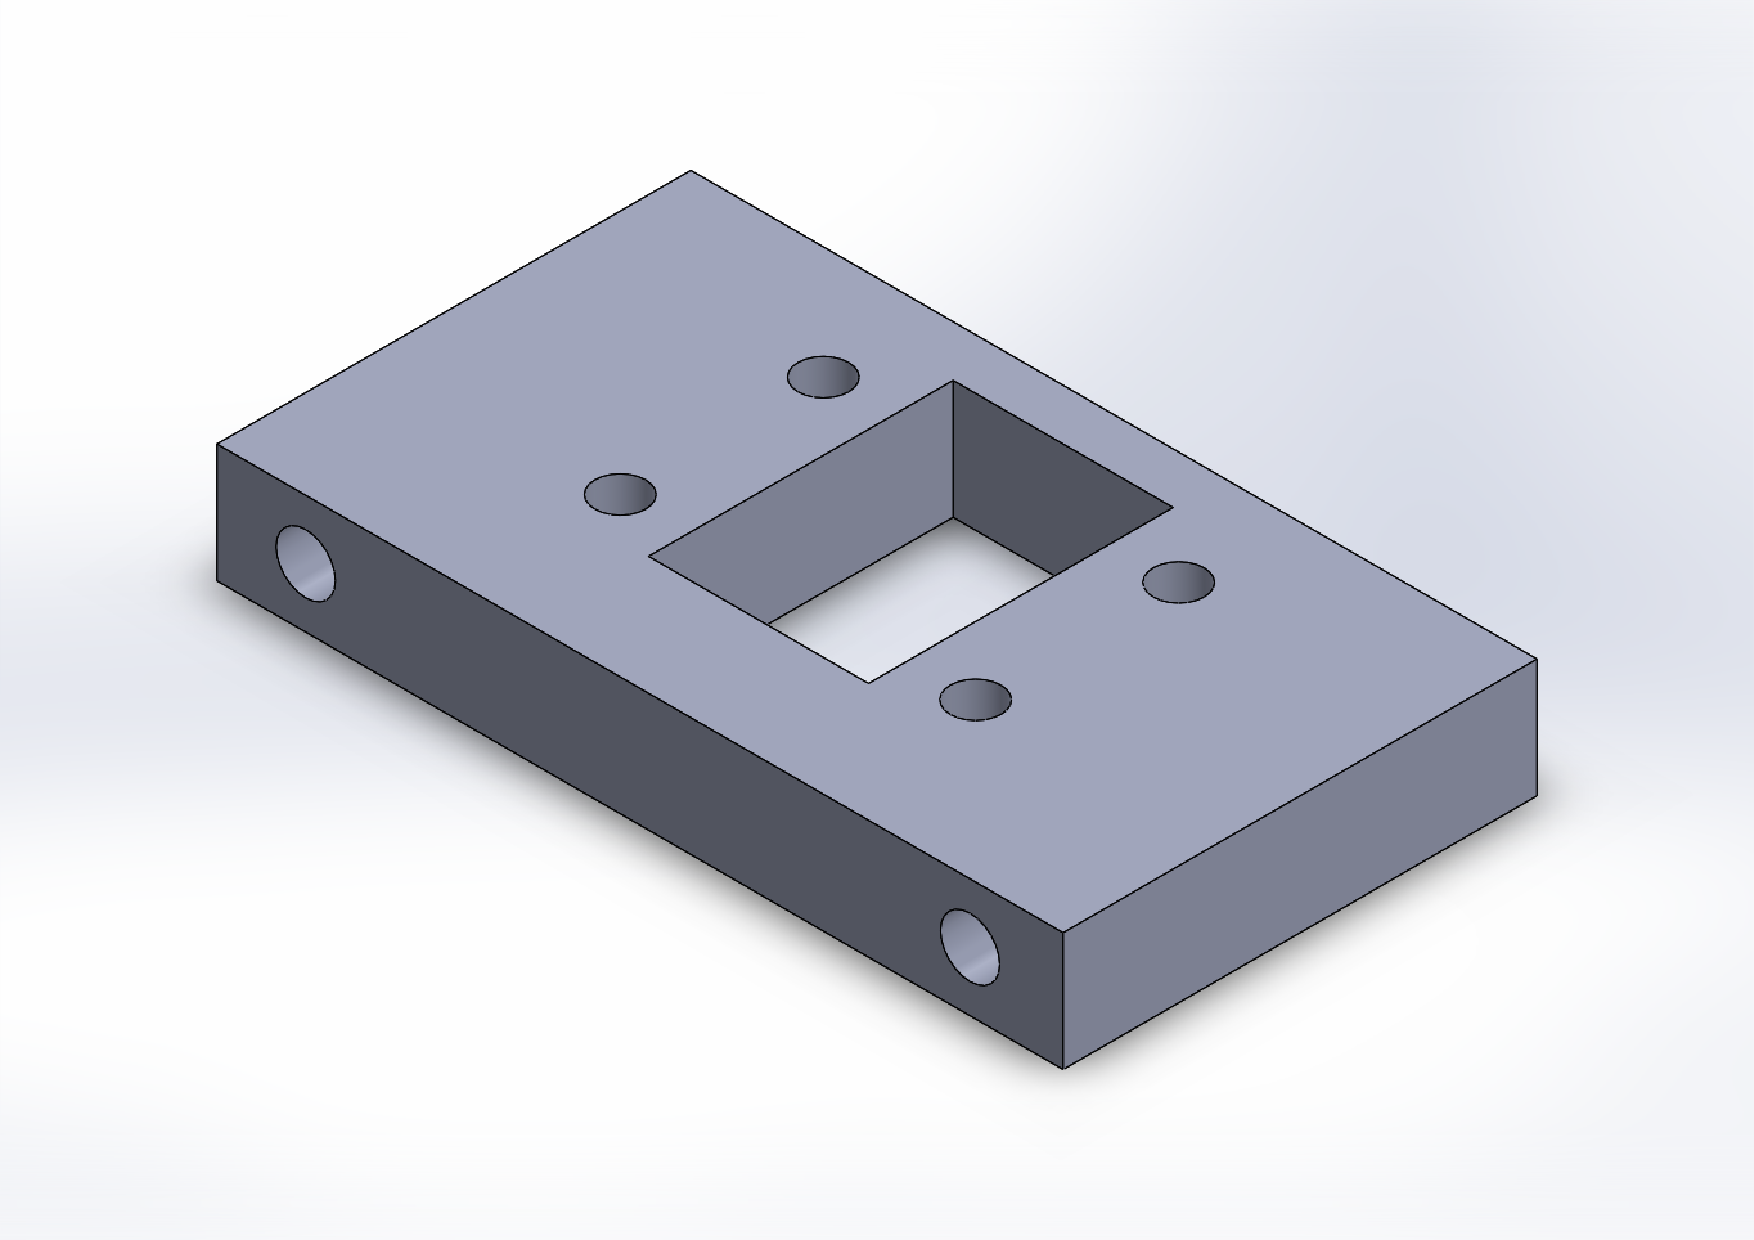
\includegraphics[scale=0.95]{../3Dmodels/camera.png}
\end{figure}

\end{changemargin}

\end{document}
